\documentclass[12pt]{article}
\title{EE445M Lab 6}
\author{Hershal Bhave (hb6279), Eric Crosson (esc625), \\
  Matt Zhan (TODO) and Robert Golshan (lol)}
\date{Friday April 10, 2015}

\usepackage[in]{fullpage}
\usepackage{listings}
\usepackage{tabularx}
\usepackage{cleveref}
\usepackage[nosolutionfiles]{answers}
\usepackage{graphicx}
\usepackage{xcolor}
\usepackage{color}
\usepackage{enumerate}
\usepackage{pdfpages}
\usepackage{float}
\usepackage{subcaption}

\newenvironment{Ex}{\textbf{Problem}\vspace{.25em}\\}{}
\Newassociation{solution}{Soln}{Answers}
\pagebreak[3]
\newcommand{\Opentesthook}[2]{\Writetofile{#1}{\protect\section{#1: #2}}}
\renewcommand{\Solnlabel}[1]{\textbf{Solution}\quad}
\newcommand{\todo}[1]{{\color{red}{\LARGE TODO} #1}}
\newcommand{\ohm}{$\Omega$}
\newcommand{\hbr}{\hfill\vspace{.25em}\\}
\newcommand{\dd}[1]{\:\mathrm{d}{#1}}
\newcommand{\ddt}[1]{\frac{\dd{}}{\dd{#1}}}
\newcommand{\dddt}[1]{\frac{\dd{}^2}{\dd{#1}^2}}

\definecolor{mygreen}{rgb}{0,0.6,0}
% \definecolor{mygreen}{rgb}{0.13,0.55,0.13}
\definecolor{mygray}{rgb}{0.5,0.5,0.5}
\definecolor{mymauve}{rgb}{0.58,0,0.82}

\lstset{
  backgroundcolor=\color{white},
  basicstyle=\scriptsize\ttfamily,
  breakatwhitespace=false,
  breaklines=true,
  captionpos=b,
  commentstyle=\color{mygreen},
  deletekeywords={...},
  escapeinside={\%*}{*)},
  extendedchars=true,
  frame=single,
  keywordstyle=\color{blue},
  rulecolor=\color{black},
  showspaces=false,
  showstringspaces=false,
  showtabs=false,
  stringstyle=\color{mymauve},
  tabsize=2,
  title=\lstname,
  columns=fullflexible,
}

\begin{document}
\maketitle

\section{Objectives}

\begin{itemize}
\item Develop a layered communication system
\item Design and implement a hardware/software interconnect protocol
\item Interface two sensors and one motor needed for the robot
\item Use communication skills to work effectively as team
\end{itemize}

\section{Hardware Design}

\begin{figure}[H]
  \centering
  \begin{subfigure}[b]{0.45\textwidth}
    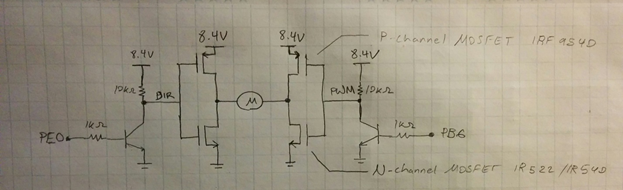
\includegraphics[width=\textwidth]{./img/motor-schematic.png}
    \caption{The MOSFET-based Motor Interface Schematic}
    \label{fig:mosfet-schematic}
  \end{subfigure}
  \begin{subfigure}[b]{0.45\textwidth}
    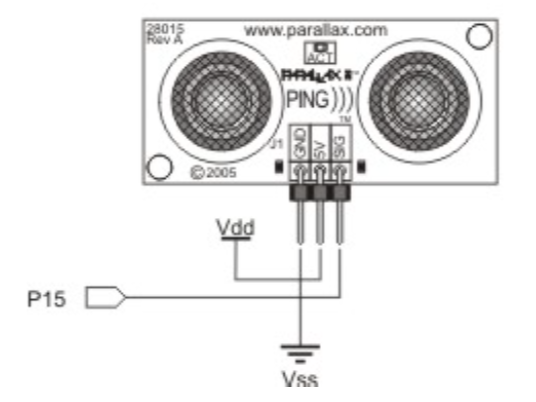
\includegraphics[width=\textwidth]{./img/ping-schematic.png}
    \caption{The Ping sensor schematic (P15 is PB0, Vdd is 5V, Vss is Gnd)}
    \label{fig:ping-schematic}
  \end{subfigure}
  \begin{subfigure}[b]{0.45\textwidth}
    \todo{IR Sensor Schematic}
  \end{subfigure}
  \caption{Lab 6 hardware interfaces}
  \label{fig:hardware-design}
\end{figure}

\section{Software Design}
Reference \cref{lst:test-can}.

\section{Measurement Data}
\begin{table}
  \centering
  \begin{tabular}{c|c|c}
    Actual distance (cm) & Sensor Measured Distance (cm) & Accuracy (\%) \\
    \hline
    2  & 3.8777 & 6.110\% \\
    3  & 2.8202 & 94.007\% \\
    4  & 3.2902 & 82.256\% \\
    5  & 4.5828 & 91.656\% \\
    6  & 5.9929 & 99.882\% \\
    7  & 6.6980 & 95.685\% \\
    8  & 7.2855 & 91.069\% \\
    9  & 8.6956 & 96.618\% \\
    10 & 10.2232 & 97.767\% \\
    11 & 11.2808 & 97.446\% \\
    12 & 12.3384 & 97.179\% \\
    13 & 13.0434 & 99.665\% \\
    14 & 14.1010 & 99.278\% \\
    15 & 15.5111 & 96.592\% \\
    16 & 16.4512 & 97.179\% \\
    17 & 17.5088 & 97.007\% \\
    18 & 18.5663 & 96.853\% \\
    19 & 19.6239 & 96.716\% \\
    20 & 20.4465 & 97.767\% \\
    21 & 21.3866 & 98.159\% \\
    22 & 22.7967 & 96.378\% \\
    23 & 23.8542 & 96.285\% \\
    24 & 24.6768 & 97.179\% \\
    25 & 25.8519 & 96.592\% \\
    26 & 27.0270 & 96.049\% \\
    27 & 27.8495 & 96.853\% \\
    28 & 28.6721 & 96.342\% \\
  \end{tabular}
  \caption{Ping Sensor Calibration}
  \label{tbl:ping-calib}
\end{table}

\begin{table}
  \centering
  \begin{tabular}{c|c}
    IR data (V) & Actual distance (in) \\
    \hline
    3.17 & 5.25 \\
    1.31 & 8.5 \\
    0.851 & 14.5 \\
    0.573 & 26.5 \\
    0.430 & 38.5 \\
  \end{tabular}
  \caption{IR Sensor (GP2Y0A21YK) Calibration}
  \label{tbl:ir-calib}
\end{table}

\begin{enumerate}
\item \todo{table of QRB1134 (motor?) data (procedure 4C)}
\item Scope traces of CAN signals are indicated in
  \cref{fig:can-frames}.
\begin{figure}[H]
  \centering
  \begin{subfigure}[b]{0.45\textwidth}
    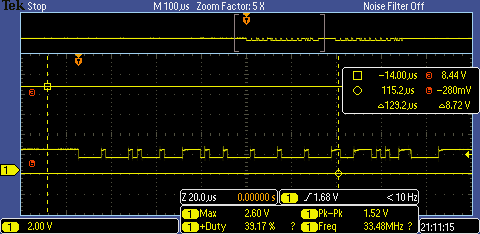
\includegraphics[width=\textwidth]{./img/TEK00008}
    \caption{CANL Signals}
  \end{subfigure}
  \begin{subfigure}[b]{0.45\textwidth}
    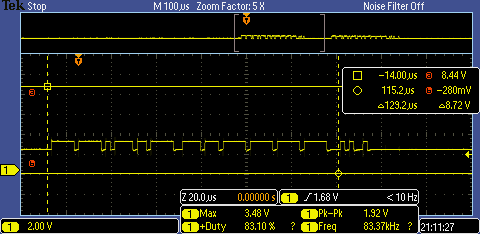
\includegraphics[width=\textwidth]{./img/TEK00009}
    \caption{CANH Signals}
  \end{subfigure}
  \caption{Scope traces of CAN signals}
  \label{fig:can-frames}
\end{figure}

\item \todo{measure network bandwidth}
\end{enumerate}

% \begin{figure}[H]
%   \centering
%   \begin{subfigure}[b]{0.45\textwidth}
%   \end{subfigure}
%   \begin{subfigure}[b]{0.45\textwidth}
%   \end{subfigure}
%   \caption{Two SPI packets}
%   \label{fig:data-frames}
% \end{figure}

\section{Analysis and Discussion}

\begin{enumerate}[1)]
\item What is one advantage of the ping sensor over the GP2Y0A21YK
  sensor? \\ \Solnlabel \newline \\
  The ping sensor is more accurate when the target is perpendicular
  and not sound-absorbant.
\item What is one advantage of the GP2Y0A21YK sensor over the ping
  sensor? \\ \Solnlabel \newline \\
  The GP2Y0A21YK provides usable distance data when the object is not
  perpendicular to the sensor.
\item Describe the noise of the GP2Y0A21YK when measured with a
  spectrum analyzer. \\ \Solnlabel \newline \\
  The data spikes at a regular interval.
\item Why did you choose the digital filters for your sensors? What is
  the time constant for this filter? I.e., if there is a step change
  in input, how long until your output changes to at least $\frac{1}{e}$ of the
  final value? \\ \Solnlabel \newline \\
  \todo{answer this question}
\item Present an alternative design for your H-bridge and describe how
  your H-bridge is better or worse? \\ \Solnlabel \newline \\
  Our H-bridge could use MOSFET transisters to reduce power leaked
  during normal operation. Our MOSFET had the advantage of requiring
  less developer time to implement.
\item Give the single-most important factor in determining the maximum
  bandwidth on this distributed system.  Give the second-most
  important factor. Justify your answers. \\ \Solnlabel \newline \\
  The most important factor in determine the maximum bandwidth of this
  distributed system is the frequency of the CAN channel, as a slow
  bandwidth is an absolute bottleneck on the system. The second
  determining factor is how quickly each component in the distributed
  system handles interrupts. This rate of interrupt handling must
  exceed the rate at which interrupts are generated.
\end{enumerate}

\newpage
\section{Code}
\lstinputlisting[language=C,label=lst:test-can,caption=\texttt{test-can.c}]{@doc-staging-area@/test-can.c}

\end{document}
